 \documentclass[a4paper,8pt]{report} %размер бумаги устанавливаем А4, шрифт 8пунктов
 \usepackage{kmanual} % собственный стиль
 \usepackage{tabularx}
 \usepackage{enumitem}
 \usepackage{graphicx}
 \usepackage{verbatim}

 \begin{document}
 \section*{Задание на разработку}
 {\tiny Версия 5}
 {\small
 \section*{«Разработка блока отвечающего за инфекционные осложнения в дневниковом осмотре»}
 \section{Введение}

 \subsection{Назначение}
    Данный документ подробно описывает доработку «ВебМИС - Стационар» в части
    блока, отвечающего за инфекционные осложнения в дневниковом осмотре. Он описывает
    общий механизм работы свойств типов действий и зависимостей между ними в рамках
    конкретного действия. Описывает ситуации, при которых необходимо прибегать к данному
    механизму и какова должна быть реакция система на действия пользователей в контексте
    указанных ситуаций. Разработчики могут использовать данный документ для реализации.

 \subsection{Границы ЗНРа}
    ЗНР описывает схему доработки базы данных и механизм работы с ней для
    выработки универсального инструмента, который позволит администраторам
    (консультантам) ВебМИС создавать произвольные системы зависимостей между
    свойствами типов действий и значениями свойств типов действий в рамках действия.

    ЗНР не содержит описание механизма администрирования взаимосвязей и
    взаимозависимостей между свойствами типа действия. Предполагается, что в конце
    реализации данного ЗНРа операции по созданию связей между свойствами типов
    действий будут осуществляться напрямую в базе данных.

    В качестве последующего ЗНРа рекомендуется описание и разработка механизма
    администрирования связей между свойствами типов действий в рамках действия.

 \subsection{Термины и определения}

 \begin{tabularx}{\textwidth}{ |X|X|X| }
    \hline
    \textbf{Термин} & \textbf{Определение}\\
    \hline
    Действие & \\
    \hline
    Свойство типа действия & \\
    \hline
    Дневниковый осмотр & \\
    \hline
 \end{tabularx}

 \subsection{Обзор документа}
    Второй раздел данного документа, «Общее описание», предоставляет общий обзор
    функциональности продукта. Он описывает формальные требования и предоставляет
    контекст для описания технических требований в следующем разделе.

    Третий раздел, «Спецификация требований», написан для разработчиков и в
    технических терминах описывает функциональность продукта.

    Оба раздела описывают один и тот же программный продукт, но на разных уровнях
    детализации и используют для этого различную терминологию.

 \section{Общее описание}
 \subsection{Системное окружение}
    В рамках данной доработки системы работают 2 типа пользователей: врач и
    администратор МИС. В роли администратора МИС может выступать консультант.

    Врач создаёт и редактирует действия, которые содержат свойства типов действий
    с взаимосвязями и взаимоограничениями.

    Администратор МИС настраивает взаимосвязи и взаимоограничения свойств типов
    действий в рамках одного действия по средствам манипуляции с БД.

 \subsection{Спецификация функциональных требований}  .
 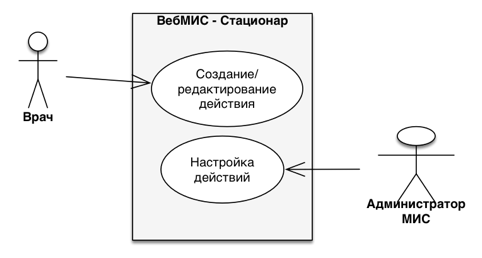
\includegraphics{roles}

 \subsubsection{Создание или редактирование действия — дневниковый осмотр (поведение при активации «Инфекционных осложнений»)}
    \paragraph*{Краткое описание}
       В разделе «Дневниковый осмотр» под раскрывающимся блоком полей «Показатели
       витальных функций» необходимо добавить раскрывающийся при установлении отметки
       блок полей «Инфекционные осложнения».

       Одно из возможных состояний при реализации данного сценария:
       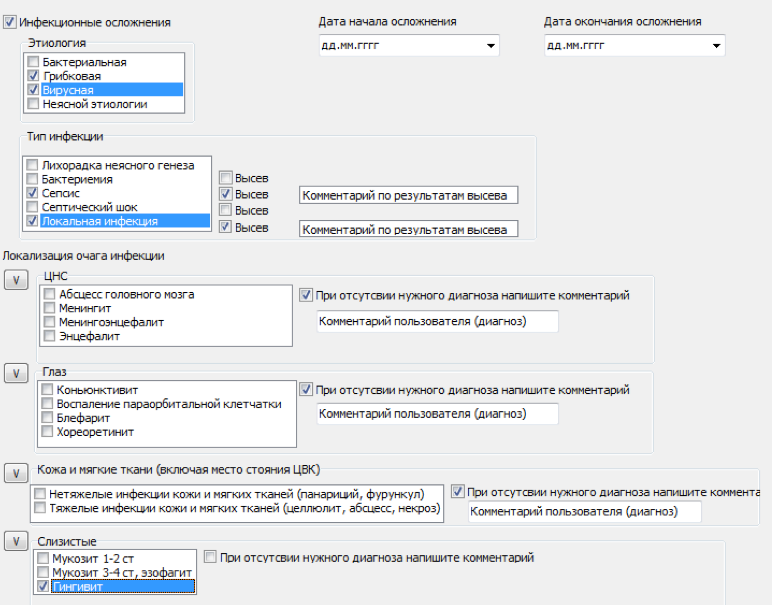
\includegraphics[width=\textwidth]{state_example}
       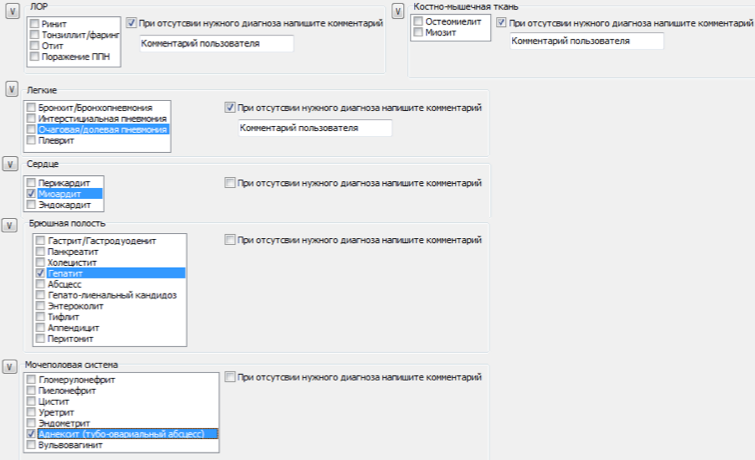
\includegraphics[width=\textwidth]{state_example_2}

    \paragraph*{Пошаговое описание}
        Предполагается, что пользователь авторизовался в системе и перешёл в раздел
        «Дневниковый осмотр».
        \begin{enumerate}
           \item Врач выбирает заинтересовавшего его пациента;
           \item В разделе «Дневниковые осмотры» («Документы») врач создает (выбирает) Дневниковый осмотр;
           \item Под раскрывающимся блоком полей «Показатели витальных функций» необходимо
                        вывести заголовок раздела «Инфекционные осложнения» (как, например,
                        "Специфическая терапия" в этом же документе). Для указания наличия осложнений
                        необходимо добавить поле "Инфекционные осложнения" с выпадающим списком
                        значений: да/нет.
           \item Если на шаге 4 выбрано значение "да", переходить к пунктам 4.1. и 4.2
              \begin{enumerate}[label*=\arabic*.]
                  \item Отображаются 2 группы флажков - «Этиология» и «Тип инфекций» со следующими
                        элементами: Этиология: бактериальная, грибковая, вирусная, неясная этиология;
                        Тип инфекции: лихорадка неясного генеза, бактериемия, сепсес, септический шок,
                        локальная инфекция. Выбор как минимум одного флажка из каждой группы -
                        обязателен. По умолчанию ни один из вариантов не выбран.
                  \item Отображаются поля «Дата начала осложнения» и «Дата окончания осложнения».
                        Поле Дата начала осложнения - обязательно к заполнению. Значение по умолчанию
                        - дата начала осложнения из предыдущего дневникового осмотра (если есть
                        предыдущий дневниковый осмотр).
                \end{enumerate}
           \item Если пользователь устанавливает флажок в одной из групп на шаге 4,
              \begin{enumerate}[label*=\arabic*.]
                 \item При проставлении флажка в группе «Тип инфекции» или «Этиология» рядом с
                       соответствующим элементом отображается флажок «Документированная
                       инфекция» (должно добавляться в тип действия как обычное текстовое поле)
                       доступный для установки. Флажок «Документированная инфекция» по умолчанию
                       не активный.
                 \item Если пользователь устанавливает флажок «Локальная инфекция» в группе «Тип
                       инфекции» на шаге 5.1, отображается группа «Локальная очаговая инфекция» со
                       следующими группами флажков: ЦНС, Глаз, Кожа и мягкие ткани (включая место
                       стояния ЦВК), Слизистые, ЛОР, Легкие, Сердце, Брюшная полость, Мочеполовая
                       система, Костно-мышечная система. По умолчанию каждая из групп флажков
                       свёрнута. Для её развертывания предусмотрен соответствующий элемент
                       управления («V»). Каждая из групп флажков содержит дополнительный флажок
                       «При отсутствии нужного диагноза напиши комментарий». Значения для каждой из
                       групп флажков приведены в Таблице «Локализации. Локальная очаговая
                       инфекция». Рядом с каждой группой «Локальная очаговая инфекция» необходимо
                       расположить поле для ввода текста со следующим комментарием: «При отсутствии
                       нужного диагноза напишите свой комментарий» (значение по умолчанию - пустое),
                       поле необязательно для заполнения.
                 \item При активации флажка «При отсутствии нужного диагноза напишите комментарий»
                      на шаге 5.3 отображается поле для ввода текста. Значение по умолчанию - пустое.
                      Комментарий к полю - «Комментарий пользователя (диагноз)»
              \end{enumerate}
           \item Пользователь выбирает сохранение либо создание дневникового осмотра.
           \item Осуществляется проверка корректности заполненности полей и сохранение изменений:
              \begin{enumerate}[label*=\arabic*.]
                 \item Если все поля заполнены верно система сохраняет данный дневниковый осмотр и
                       возвращает пользователя к перечню документов (дневниковых осмотров).
                 \item Если какого-либо из полей заполнено некорректно система сообщает пользователю
                       какое именно и предлагает осуществить коррекцию.
              \end{enumerate}
        \end{enumerate}

    \paragraph*{Таблица. Локализации. Локальная очаговая инфекция.}
        \begin{tabularx}{\textwidth}{ |X|X|X| }
            \hline
            ЦНС  & Абсцесс головного мозга, Менингит, Менингоэнцефалит, Энцефалит                           \\ \hline
            Глаз & Коньюнктивит, Воспаление параорбитальной клетчатки, Блефарит, Хореоретинит               \\ \hline
            Кожа и мягкие ткани (включая место стояния ЦВК) & Нетяжелые инфекции кожи и мягких тканей
                (панариций, фурункул), Тяжелые инфекции кожи и мягких тканей (целлюлит, абсцесс, некроз)    \\ \hline
            Слизистые & Мукозит 1-2 ст, Мукозит 3-4 ст, эзофагит, Гингивит                                  \\ \hline
            ЛОР & Ринит, Тонзиллит/фарингит, Отит, Поражение ППН                                            \\ \hline
            Легкие & Бронхит/бронхопневмония, Интерстициальная пневмония, Очаговая/долевая пневмония,
                Плеврит                                                                                     \\ \hline
            Сердце & Перикардит, Миоардит, Эндокардит \\
            Брюшная полость & Гастрит/гастродуоденит, Панкреатит, Холецистит, Гепатит,
                Гепато-лиенальный кандидоз, Абсцесс , Энтероколит, Тифлит, Аппендицит, Перитонит            \\ \hline
            Мочеполовая система & Гломерулонефрит, Пиелонефрит, Цистит , Уретрит, Эндометрит, Аднексит
                (тубо-овариальный абсцесс), Вульвовагинит                                                   \\ \hline
            Костно-мышечная система & Остеомиелит, Миозит                                                   \\
            \hline
         \end{tabularx}
 \subsubsection{Создание или редактирование действия — дневниковый осмотр (поведение при активации «Терапии»)}
    \paragraph*{Краткое описание}
        В разделе «Дневниковый осмотр» при установке флажка «Терапия» помимо текстового
        поля должна быть предусмотрена возможность выбора вида терапии и медикаментозного
        назначения для каждого из видов терапий.

        Одно из возможных состояний при реализации данного сценария:
        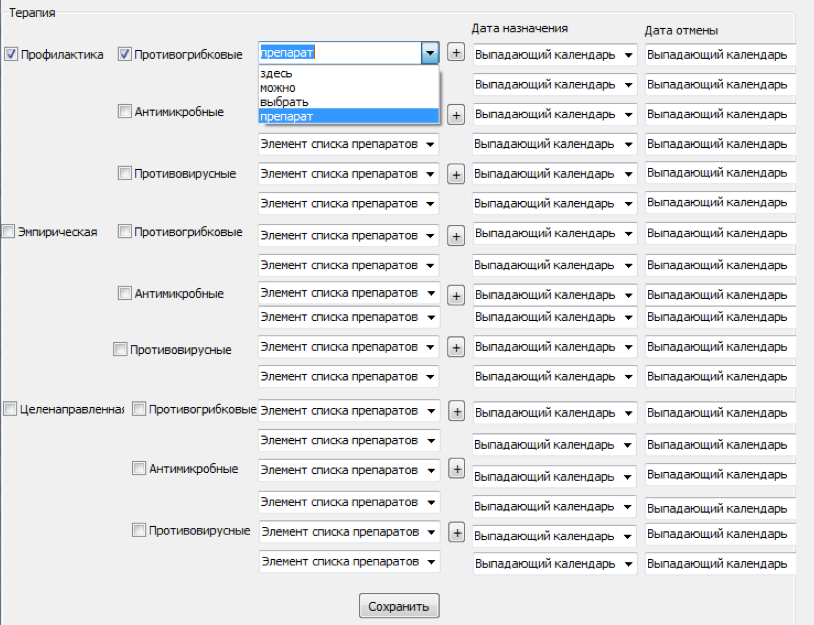
\includegraphics[width=\textwidth]{state_example_3}

    \paragraph*{Пошаговое описание}
        Предполагается, что пользователь авторизовался в системе и перешёл в раздел
        «Дневниковый осмотр».

        \begin{enumerate}
              \item Врач выбирает заинтересовавшего его пациента;
              \item В разделе «Дневниковые осмотры» («Документы») врач создает (выбирает)
              Дневниковый осмотр;
              \item При установке флажка «Терапия» отображается блок флажков со следующими
              значениями (типами терапий): Профилактика, Эмпирическая, Целенаправленная. По
              умолчанию ни один из флажков не проставлен. Допускается сохранение дневникового
              осмотра если ни один из флажков не выбран.
              \item Пользователь устанавливает флажки напротив наименования необходимого типа
              терапии.
              \item Напротив установленного на шаге 4 типа терапии отображается список флажков
              группы препаратов со следующими значениями: противогрибковые, антимикробные,
              противовирусные. По умолчанию все флажки не проставлены.
              \item Пользователь устанавливает флажки напротив необходимой группы препаратов.
              \item После проставления на шаге 6 необходимой группы препаратов становится доступной
              кнопка выбора препарата.
              \item При нажатии на кнопку выбора препарата на шаге 7 отображается выпадающий список
              препаратов. При выборе препарата препарат назначается. Данную операцию можно
              повторять неограниченно количество раз. Необходимо предусмотреть возможность
              удаления выбранного препарата.

              Доступные по умолчанию, т.е. такие, которые отображаются в выпадающем списке,
              препараты для группы \textbf{«Противогрибковые»}: Амбизом, Амфолип, Вифенд, Кансидас,
              Микамин, Ноксафил, Флюконазол, Дифлюкан,Микосист, Эраксис.
              Доступные по умолчанию в группе \textbf{«Антимикробные»}: Амикацин, Амоксициллина
              клавуланат, Аугментин, Амоксиклав, Бисептол, Ванкомицин, Эдицин, Дориппрекс,
              Зивокс, Зиннат, Изониазид, Кларитро/Азитромицин, Клиндамицин, Колистин,
              Максипим, Меронем, Метронидазол, Флагил, Метроджил, Панцеф, Роцефин,
              Сульперазон, Тазоцин, Тиенам, Фортум, Фторхинолоны.

              Доступные по умолчанию в группе \textbf{«Противовирусные»}: Зовиракс, Ацикловир,
              Цимевен.

              Помимо этого в каждом списке доступен выбор препарата «Другое» (в самом конце
              списка).

              Если выбран «Другое», тогда пользователю необходимо отобразить поле для ввода
              текста. Значение по умолчанию - пустое. Комметарий к полю - «Введите наименование
              препарата». Допускается пустое значение при сохранении.

              \item При назначении препаратов на шаге 8 назначенные препараты отображаются напротив
              соответствующей с шага 6 группе препаратов.
              \item При назначении препарата и схемы его приема на шаге 8 рядом с наименованием
              препарата становятся доступными для заполнения поля «Дата назначения» и «Дата
              отмены» в виде выпадающего календаря. Оба поля по умолчанию пустые и являются
              обязательными для заполнения.
              Если существует предыдущая дневниковая запись, а текущая - новая (создаётся),
              тогда значением по умолчанию поля «Дата назначения» принимает значение «Даты
              назначения» предыдущей записи такого же типа для данного пациента.
              Если предыдущая дневниковая запись помимо даты назначения содержит и дату
              отмены, тогда из предыдущего дневника дата не заполняется и не копируется
              наименование соответствующего препарата.
              \item Пользователь выбирает сохранение либо создание дневникового осмотра.
              \item Осуществляется проверка корректности заполненности полей и сохранение
              изменений:
              \begin{enumerate}[label*=\arabic*.]
                \item Если все поля заполнены верно система сохраняет данный дневниковый осмотр и
                возвращает пользователя к перечню документов (дневниковых осмотров).
                \item Если какого-либо из полей заполнено некорректно система сообщает пользователю
                какое именно и предлагает осуществить коррекцию.
              \end{enumerate}
           \end{enumerate}
 \section{Спецификация требований}
 \subsection{Требования к интерфейсу}
    Так как описанный ниже механизм работы с зависимыми свойствами типов действий
    будет описан ниже, а его релазиция будет осуществляться в нескольких программных
    компонентах в процессе разработки интерфейса необходимо опираться на правила,
    принятые для конкретного программного компонента и на схемы интерфейса,
    приведенные в разделе 2.2.1 и 2.2.2 данного документа.
 \subsection{Функциональные требования}
 \subsection{Нефункциональные требования}
 \subsubsection{Модификация логической структуры данных}
    В рамках данной доработки необходимо модифицировать существующие структуры
    данных. В частности, база данных должна хранить информацию, которая позволит на
    уровне бизнес логики:
    \begin{itemize}
       \item указывать, при каких условиях необходимо отображать свойство типа действия в
    зависимости от состояния другого свойства типа действия;
       \item указывать, при каких значениях свойства типа действия необходимо отображать
    зависимое свойство типа действия.
    \end{itemize}

    В данном разделе термин «показывать» и «делать доступным» подразумевает одно и то
    же и зависит исключительно от конкретного интерфейсного решения.

    Пусть даны 3 свойства типа действия: A, B и С.
    База данных должна хранить информацию, которая позволит осуществлять следующие
    переходы между состояниями:

    \paragraph*{Переходы между состояниями №1:} Показывать B, когда A - истина.
    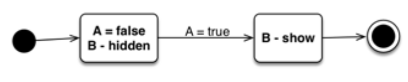
\includegraphics{condition_1}

    \paragraph*{Переход между состояниями №2:} Показывать С, когда А - истина, B - истина.
    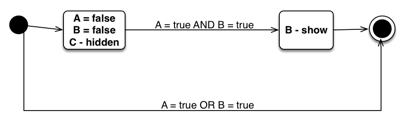
\includegraphics{condition_2}

    Как видно из \textbf{Переходов между состояниями 1 и 2} условия перехода можно
    масштабировать на произвольное количество зависимостей между свойствами типой
    действий.

    \paragraph*{Переход между состояниями №3:} Показывать В когда А - истина и А = Значение\_1
    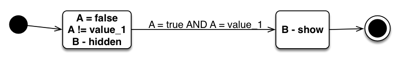
\includegraphics{condition_3}

    \paragraph*{Переход между состояниями №4:} Показывать С когда А - истина и А = значение\_1 и В - истина и В = значение\_2
    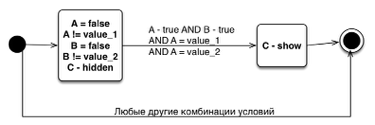
\includegraphics{condition_4}

    Как видно из Переходов между состояниями 3 и 4 условия перехода можно
    масштабировать на произвольное количество зависимостей и значений между свойствами
    типов действий.

    Бизнес-логика приложения должна реализовывать переходы между соответствующими
    состояниями.

    Для этого базу данных необходимо дополнить следующими таблицами:
    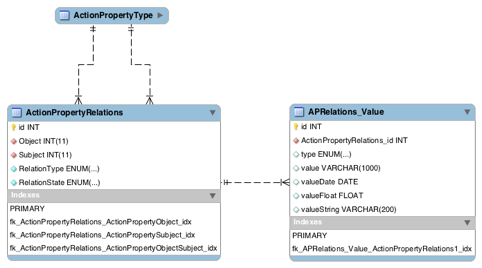
\includegraphics{table_structures}

    Код для создания новых таблиц в существующей схеме:
\begin{verbatim}
CREATE TABLE IF NOT EXISTS `ActionPropertyRelations`
    ( `id` INT NOT NULL AUTO_INCREMENT,
    `Subject` INT(11) NOT NULL COMMENT 'Ссылка на родительское свойство
        типа действия.',
    `Object` INT(11) NOT NULL COMMENT 'Ссылка на дочернее свойство типа
        действия',
    `RelationType` ENUM('bool', 'equals', 'in', 'nin', 'lt', 'gt')
        NOT NULL COMMENT
    'bool - для логических условий (True)
    equals - для точного совпадения значений (=)
    lt - меньше чем(<)
    gt - больше чем (>)
    has_value - имеет значение
    in - в каком-то множестве значений
    nin - не в каком-то множестве значений',
    `RelationState` ENUM('show', 'available', 'required') NOT NULL COMMENT '
    show - показать свойство типа действия
    available - сделать доступным свойство типа действия
    Доступность - это подмножество понятия "показать".
    Можно сначала показать, потом сделать доступным (например, для выбора
        или редактирования)
    required - обязательно для заполнения',
    PRIMARY KEY (`id`),
    INDEX `fk_ActionPropertyRelations_ActionPropertyObject_idx`
        (`Object` ASC),
    INDEX `fk_ActionPropertyRelations_ActionPropertySubject_idx`
        (`Subject` ASC),
    INDEX `fk_ActionPropertyRelations_ActionPropertyObjectSubject_idx`
        (`Object` ASC, `Subject` ASC),
    CONSTRAINT `fk_ActionPropertyRelations_ActionPropertyObject`
        FOREIGN KEY(`Object`)
        REFERENCES `ActionPropertyType` (`id`)
        ON DELETE CASCADE ON UPDATE CASCADE,
    CONSTRAINT `fk_ActionPropertyRelations_ActionPropertySubject`
        FOREIGN KEY (`Subject`)
        REFERENCES `ActionPropertyType` (`id`)
        ON DELETE CASCADE ON UPDATE CASCADE) ENGINE = InnoDB;

    CREATE TABLE IF NOT EXISTS `APRelations_Value` (
    `id` INT NOT NULL AUTO_INCREMENT,
    `ActionPropertyRelations_id` INT NOT NULL
        COMMENT 'Ссылка на запись в таблице отношений между аттрибутами
        {ActionPropertyRelations}',
    `type` ENUM('flatDirectory', 'Action', 'Event') NULL DEFAULT NULL
        COMMENT 'Тип ссылки на другую таблицу или объект.',
    `valueReference` int(11) NULL DEFAULT NULL
        COMMENT 'Значение ссылки на другую таблицу или объект.',
    `valueDate` DATE NULL DEFAULT NULL
        COMMENT 'Поле, если значение является не ссылкой на
        другой объект и имеет тип - дата.',
    `valueFloat` FLOAT NULL DEFAULT NULL
        COMMENT 'Поле, если значение является не ссылкой на
        другой объект и имеет тип - число.',
    `valueString` VARCHAR(200) NULL DEFAULT NULL
        COMMENT 'Поле, если значение является не ссылкой на
        другой объект и имеет тип - строка.',
    PRIMARY KEY (`id`),
    INDEX `fk_APRelations_Value_ActionPropertyRelations1_idx`
    (`ActionPropertyRelations_id` ASC),
    CONSTRAINT `fk_APRelations_Value_ActionPropertyRelations1`
    FOREIGN KEY (`ActionPropertyRelations_id`)
    REFERENCES `ActionPropertyRelations` (`id`)
    ON DELETE CASCADE ON UPDATE CASCADE) ENGINE = InnoDB;
\end{verbatim}

    \paragraph*{Описание таблицы ActionPropertyRelations}
    \begin{tabularx}{\textwidth}{ |X|X|X| }
        \hline
        \textbf{Название} & \textbf{Тип} & \textbf{Комментарий} \\
        \hline
        id      &   INT     &   Ключевое поле для индексации \\
        \hline
        Object  &   INT(11) &   Объект, относительно которого формируется зависимость. \\
        \hline
        Subject &   INT(11) &   Субъект, для которого формируется зависимость от объекта \\
        \hline
        RelationType & ENUM('bool', 'equals', 'lt', ‘gt’, ‘in’, ‘nin’) &
            bool - для логических условий (True)
            equals - для точного совпадения значений (=)
            lt - меньше чем (<)
            gt - больше чем (>)
            in - является одним из элементов
            nin - не является одним из элементов \\
        RelationState & ENUM('show', ‘available’,
        ‘required’) &
            show - показать свойство типа действия
            available - сделать доступным свойство типа действия
                Доступность - это подмножество понятия "показать". Можно сначала показать, потом сделать доступным
                (например, для выбора или редактирования)
            required - поле является обязательным для заполнения \\
        \hline
     \end{tabularx}

    \paragraph*{Таблица APRelations\_Value}
    \begin{tabularx}{\textwidth}{ |X|X|X| }
            \hline
            \textbf{Название} & \textbf{Тип} & \textbf{Комментарий} \\
            \hline
                id & INT & Ключевое поле для индексации \\ \hline
                ActionPropertyRelations\_id & INT & Ссылка на ActionPropertyRelations \\ \hline
                type & ENUM('flatDirectory', 'Action', 'Event') & Тип ссылки на другую таблицу или объект. \\ \hline
                value & VARCHAR(1000) & Значение ссылки на другую таблицу или объект. \\ \hline
                valueDate & DATE & Поле, если значение является не ссылкой на другой объект и имеет тип - дата. \\ \hline
                valueFloat & FLOAT & Поле, если значение является не ссылкой на другой объект и имеет тип - число. \\ \hline
                valueString & VARCHAR(200) & Поле, если значение является не ссылкой на другой объект и имеет тип - строка. \\
            \hline
         \end{tabularx}

    Примеры реализации переходов между состояниями на основе новой таблицы:
 }
 \end{document}
